%%%%%%%%%%%%%%%%%%%%%%%%%%%%%%%%%%%%%%%%%%%%%%%%%%%%%%%%%%%%%%%
%
% Welcome to the PPIP Documentation.
% This document is to help you access all the resources of the ppip system with ease.
% The document begins with the chapter on the overview of the system.
% This is followed by a description of the public side as well as the private facing side of the system.
% On the public side we discuss the various sections tenders contracts, suppliers, and procurement Entities.
% The private side begins with the registration of a procuring entity then the login process of the procurement entity followed by the dashboard then the side panel then a deep dive into the various submodules.

% The Submodule each define their purpose in PPIP then their use in real procurement and how they can be used procedurally.
% The module are divided to start with the PE then the Compliance officer followed by the admininstrator last.

% As a result the modules are not in the normal order but follow this pattern, the administrator modules are not found in this user guide but in the administrators guide for managing, troubleshooting and supporting the system and its users.


%
%%%%%%%%%%%%%%%%%%%%%%%%%%%%%%%%%%%%%%%%%%%%%%%%%%%%%%%%%%%%%%%
\documentclass [12pt]{book}

\usepackage{graphicx}
\usepackage{hyperref}
\usepackage{wrapfig}

\graphicspath{{./private_images/}{./public_images/}}

\title{THE PPIP MANUAL}
\author{The PPIP Development Team}
\date{July 2024}

% preamble end

\begin{document}

\maketitle


\chapter{Getting Started}
The Procurement Information Portal is the offical reporting platform for all procurment activities of a procuring entity.\\
The platform allows all procuring entities to report their procurement activities to the public procurement regulatory authority PPRA and makes their tenders, contracts and procurement activities readily available to the public allowing them to particapate in the procurement process as and provide oversight.\\

To get started with the platform:\\

    \begin{enumerate}
    
    \item Go to \url{https://tenders.go.ke}
    
    \begin{figure}
        
\includegraphics[scale = 0.25 ]{public_images/landing_page.png}
        \caption{PPIP: Landing Pege}
        \centering
    \end{figure}
    
    \item If you don’t have an  account yet
\section {Create an Account}

As a Procuring Entity (PE) one can get started with the platform by creating a procurement entity account. This account allows a PE to report all their procurement activities on the platform.\\
This account is an organizational account and requires the PE to first search for their account as most PEs are already registered on the platform. However in case their iss not account the PE can register for an account on the platform. After filling in the application PPRA will review the application. Once PPRA verifies the details of the PE the PE account will be created and a link will be sent to the account holder via email.\\

To create an account:\\ 
    
    \begin{enumerate}    
        \item Go to the PPIP platform on http://www.tenders.go.ke.
       \begin{figure}[h]
        
\includegraphics[scale = 0.25 ]{public_images/landing_page.png}
        \centering
        \caption{PPIP: Landing Pege}
    \end{figure}
    
        \item click PE Registration on the top right hand side of the screen.
        This will open the registration section.
        % [image]
        
        \begin{figure}
            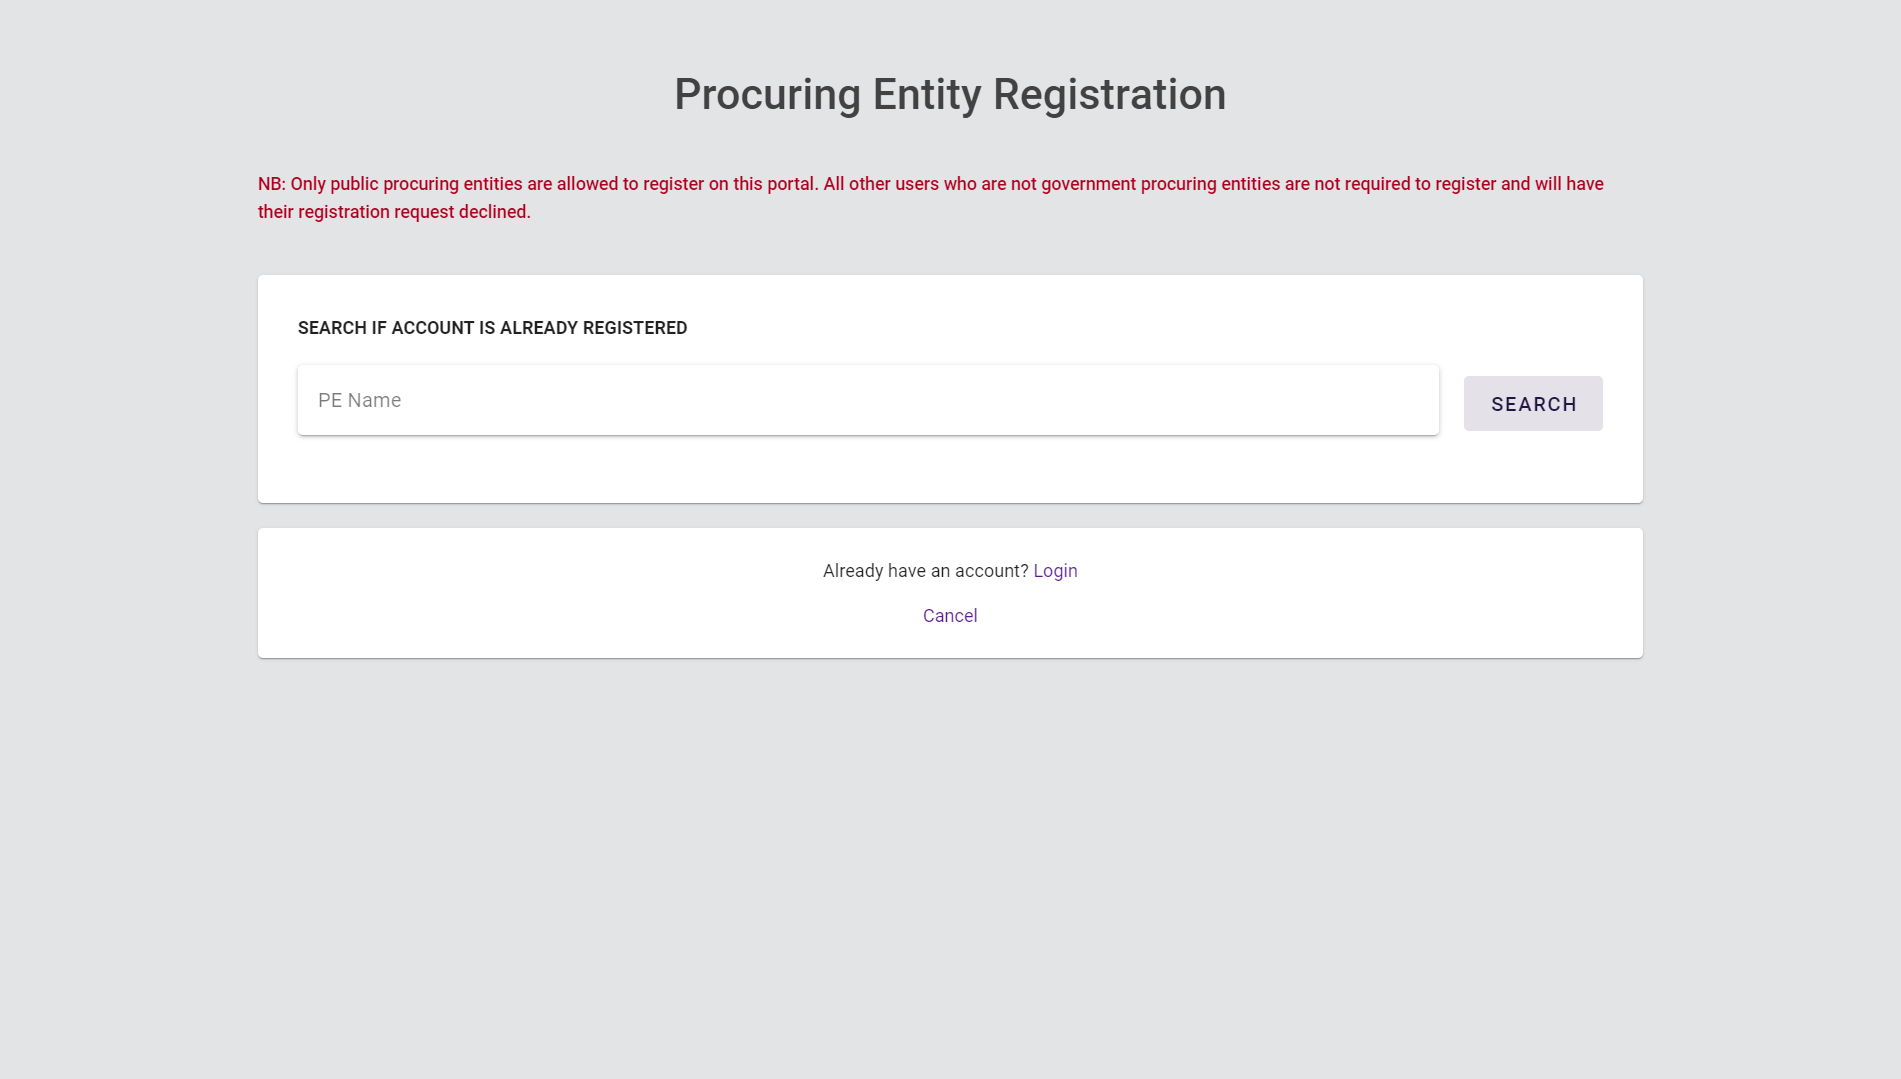
\includegraphics[scale=0.25]{public_images/registration_page.png}
            \caption{registration page}
            \centering
        \end{figure}
        
        \item Enter your Procuring Entity's name to search if a PE account already exists.
        
        If no account exists a button appears for registration
        \begin{enumerate}
            \item Click No data found for your search. Click here to register now!
            % [image]
        \end{enumerate}

        This will open the registration form\\
        \item complete the registration form and submit.
        \item notifications are sent to submitted emails throughout the process from email verification, approval request, and approval at which point the user can log-in
    \end{enumerate}


In case a PE account is present then to login to the account:\\ 

    \begin{enumerate}
        \item click PE Login
        \item Enter your email.
        \item Enter your password.
    \end{enumerate}

In case the account password has been forgotten then use the forgotten password link the login page:

    \begin{enumerate}
        \item	Go to the Login page 
        \item	Click on “Forgot your password?”
        \item	Enter your valid account email address 
        \item	click Submit
        \item	A password reset link will be sent to your email.
        \item	Check your email 
        \item	Follow the reset link to reset your password.
    \end{enumerate}

\end{enumerate}
\clearpage

\chapter{The PE Dashboard}

Once logged in as a procurement entity you will be able to manage all your procurement activities.
To access activities, click on the menu icon on the top left corner of your screen.
This will open the sidebar that has all the procurement activities you can do.
Each procurement activity is under a category the categories are as follows:

\section{Sidebar Layout}
Access the sidebar by clicking on the menu icon on the top left-hand side of the screen.

This will reveal the sidebar with all the sections that can be done by a user.
The sections are organized in modules:


Each module has a specific purpose follows:

Click on a module to expand the modules to find specific sections.
For example, the operation Module Expands like so:


To work with the system effectively it will be prudent to know where each section is.
For reference here is a list of all the different Modules and their sections as well as their uses:

User Management:
[Table]


Configurations:
[Table]


Operations module:
[Table] 


Listings module:
[Table]

Compliance Module:
[Table]

Notices:
[Table]

Generate Report:
[Table]


Announcements:
[Table]

\section{Operations Module}
The operations module is the primary workspace for most procurement processes.
It is for creating and managing all procurement operations, including managing tenders, contracts, Framework Agreements, Low Value Procurements and Disposals (of Assets, to Employees and by Public Auctions).

\subsection{Procurement Plans}
To begin the procurement process the PE must first create and publish their procurement plan.

To create a procurements plan on the system:
\begin{enumerate}
\item Navigate to the operations module 
\item Click on draft procurement plans 
\item Click upload procurement plan 


In case, there is no existing procurement plan, download and fill the procurement plan template, then click upload procurement plan.

\item Fill in the procurement plan form with the necessary details, the financial year of the procurement plan the total procurement budget the total reserve for AGPO and indicate amendment to show if it is an amendment to an existing procurement plan select amendment.

\item Click approval from accounting officer to upload the approval document  
\item Select the file from your machine
\item In the same way upload the procurement plan document however note only excel files are allowed.
\item Once your form is filled click save.
\item The procurement plan will be saved as a draft procurement plan, which can be edited as needed.
\item Once satisfied with the draft procurement plan publish the plan: 
\item Click on actions 
\item Click on publish 
\item Fill in the details of the publication
\item Upload the necessary documents 
\item Click publish
\item The procurement plan will be placed into the published procurement plan page.
\end{enumerate}


\subsection{Create Tenders Module}
To Create a Tender use the Create Tender section as follows:
\begin{enumerate}
\item 	Open the sidebar in the operations section 
\item 	Click on create Tender module
\item 	Fill out the create tender form.  
\item 	The form has various fields as follows: 
To make a tender an AGPO / Preference and Reservation Scheme (Youth, Women and People with Disabilities) tender.
\item 	Click the checkbox marked “Is Tender for Preference and Reservation Scheme”
Like so, choose the appropriate group
For Example: 
AGPO (Youth, Women, PWDs)

\item 	Attach the tender documents (NB: Tender Document is a mandatory attachment).
\begin{enumerate}
\item 	Choose document type:
 
\item 	Type a description for the document you have selected.
\item 	Click the Attach File field to navigate to the document on your computer,
 
\item 	To attach additional documents, click on the Attach New Document button
 
\item 	Then repeat the process, to add all your documents.
 
\end{enumerate}

\item 	Click Save Draft to save the tender notice as a draft.
\end{enumerate}



\subsection{Draft Tenders}
The draft Tenders Section displays all draft tenders.
A tender once created is first saved to the draft tenders section. 
This allows for editing, as at this point the tender is not yet visible to the public.

A user can perform four major actions:
\begin{enumerate}
\item	View to see the details
\item	Edit to modify the draft tender 
\item	Publish to mark the tender as published 
\item	Delete to delete the tender
\end{enumerate}

To use actions in the system 
\begin{enumerate}
\item	Go to draft tenders section under operations.
\item	Click more actions on the specific tender.
\end{enumerate}


To edit a draft tender :
\begin{enumerate}
\item	Click edit under more actions
\item	Edit the tender using the edit menu that will appear.
\item	Make all the tender as desired
\item	Click save
\end{enumerate}

2.	To publish the draft tender:
\begin{enumerate}

\item Click publish on More Actions
\item Confirm the publication on the pop up that will appear
Note: Publish will mark the tender as published and move it to the published tenders section. 
Once the tender is published it is moved to the “Published Tenders” section and becomes visible to the Kenyan public on the PPIP Home Page.
 
\end{enumerate}
3.	To delete the draft tender:
\begin{enumerate}
    \item Click delete under More Actions
\end{enumerate}
Note: deleting a tender is not reversable so beware and use it sparingly.
To prevent accidental deleting a pop-up will appear to ask for confirmation, on whether to delete or not to delete.




\subsection{Published Tenders}
Once a tender is published you will see it in published tenders.
This page displays the all tender Details with a tenders status, to track it’s progress. Here is an example of how to use published tenders.

Accessing Published Tenders
\begin{enumerate}
\item	Access published tenders from the side-menu item Published Tenders
NB: The status of the tender will be “Not Complete” meaning that the tender has not been fully reported up to completion e.g. contract award, termination, etc.

\item	Perform actions by clicking “Actions” then a small menu will open with View more details, Add more details, Add Addendum, or Terminate.
These options will let you work on your tender:
\begin{enumerate}
\item	View more details: See published tender Details 
\item	Add more details: Add to published tender and make it progress
\item	Add Addendum: Add an addendum in case of any changes
\item	Terminate: Mark the tender as terminated and End its progress.
\item	Documents: View all Tender Documents needed.
\end{enumerate}

Note: Once Terminated a tender cannot be edited or added to.
\end{enumerate}

\subsection{Operating on Published Tenders}
\begin{enumerate} 
\item	View More Details
    \begin{enumerate}
    \item	Click the Actions button then choose View More Details.
    \item	Review Tender Details.
    \item	Close tender dialog.
    \end{enumerate}

\item	Add Addendum
    \begin{enumerate}
    \item	Click the Actions button then choose Add Addendum.
    \item	Fill in the Addendum Form then click Submit.
    \end{enumerate}
    NB: Addendum does not have a save to draft option and is published immediately after it is submitted.


\item	Terminate Tender
    \begin{enumerate}
        \item	Click the Actions button then choose Terminate.
        \item	Fill in the Termination Form
        \item	Add all the documents needed then click Submit.
        \item	Confirm you want to terminate the tender.
    \end{enumerate}
    NB: Once Terminated a tender cannot be edited or added to.
    Take care not to terminate a tender accidentally be sure the tender you are terminating is the correct tender. In extreme circumstances, you can contact the system administrator to seek help with the terminated tender.

\item Documents 
    \begin{enumerate}
        \item	Click the Actions button then choose Documents.
        \item	Review the Tender document and click Close.
    \end{enumerate}

\item	Adding More Details to Tender
    \begin{enumerate}
        \item Click the Actions button then choose Add more details.
        \item This will open the published tender allowing you to add to and make it progress.
    \end{enumerate}
    
\item Adding Details to Published Tender from Opening, Evaluation to Award

\begin{enumerate}
\item In the Published Tenders section, click the Actions button.
\item Choose Add more details.
This will open the add details menu to update the details of the tender, form opening, evaluation, contract till inspection.
The tender Details menu is detailed in this section:
\end{enumerate}

\subsection {Published Tender 2\\ Adding More Details To A Published Tender}

The tender details menu capture the tender creation and update process.
It splits the tender process into 4 sections Tender Opening, Evaluation, Contracts and Evaluation.
Each section is a step in the tender process and ahs its own use capturing different documents.
In a regular open tender the steps are :
\begin{enumerate}
\item Tender Opening
\item Bidder Evaluation
\item Contract  
\item Evaluation
\end{enumerate}

These steps will be referred to by number e.g Step 1: Tender Opening, and Step 4: Evaluation. 

Details of the various sections as follows: \\
\begin{enumerate}
\item{Step 1: Tender opening} \\
        This covers the opening phase of the tender the bidders that applied for the tender are added as well as the required tender opening minutes and supporting documents. \\


Note: To progress in the tender details menu complete Step 1: Tender Opening, by filling in the details relating to how the tender was opened as follows:

\begin{enumerate}
    \item	Fill in the details of the bidder who participated in the tender, once filled in click add bidder. 
    The bidder is added to the tender and appears below the form. Repeat this for all bidders in the tender. Once complete it will appear like so:
    % [Image]
    
    \item Alternatively in case of many bidder, create a filled bidders template by:

       - Clicking Download Template, to download an empty bidders template. 
    Note Do not use formulas only use real values or drag down and duplicate values but not avoid formulas for the bidder template.
    Fill in the empty bidders template like so and save it in a easily to remember folder.

    \item Fill in the opening date of the tender.
    Click attach Excel file and select the filled bidders file that was previously saved.
    
    All the bidders will appear under the form like so:
    \item Attach the necessary documents e.g.Tender Opening Minutes, as shown: 
    
    \item Once you are done, click the continue button to move to Step 2. 
\end{enumerate}

\item {Step 2: Evaluation}, \\
This stage specifies the outcomes of the evaluation stage by recording bidder performance.

\begin{enumerate}
    \item Capture the evaluation outcomes by filling the sections for Preliminary Evaluation, Technical Evaluation, and Financial Evaluation.
    
    \item Check the checkbox for the bidders who passed the respective stages.
    \item Uncheck for those who did not pass.
    \item Where scores are required, fill in what the bidder scored (in addition to checking the checkbox).
    \item In case there were no scores, leave it blank but make sure you tick the bidders who passed.
\item Capture the details of the evaluation committee members by selecting the names of the members who participated in the evaluation.
 
i.	NB: If the name of any member is not in the list they can be added under the User Management section.
ii.	Once this is done, attach and upload the relevant documents e.g. Evaluation report,
iii.	Click “Continue” to move to the next section (Step 3).
\end{enumerate}


\item{Step 3: Contract}
This is the section where passed bidders are awarded contracts for the tender.
Only bidders that passed evaluation will appear on the supplier selection menu.
To award a contract:

\begin{enumerate}
    \item Select the name of the bidder who was awarded the tender
    \item If validated name does not autofill, click the Validate New Supplier button to verify the bidder details with the BRS (Business Registration Services) database.
    \begin{enumerate}
        \item Enter the Business Registration number (Certificate of Registration/Incorporation number) in the Suppliers form then click “Validate”.
        \item The system will validate the details of the supplier against the BRS database and retrieve the correct details of the supplier.
        \item Fill in the remaining details e.g email, PIN etc.
        \item Click “Save Supplier Details” then add the Beneficial Ownership Details. (Not applicable for Requests For Quotations (RFQs) )
        \item Enter the details of all the beneficial owners of the firm (As provided in Form No. 8 – Beneficial Ownership Disclosure Form)
        \item then click “Save Validated Supplier Details”
        \item You will then be returned to the contract form and be required to fill in the the remaining details
    \end{enumerate}
    
    \item Once you have captured the contract details click the “Save Contract Details” button to save the contract.
    \item Upload the appropriate documents e.g Contract, LPO/LSO then close.\\
    The contract will be moved to the draft contracts section where it can be reviewed before being published.
    Please note that a draft contract can be edited and deleted but cannot be altered after publishing, just like the draft tenders stage when creating a tender. 
\end{enumerate}
    
    


\subsection{Contracts}
The Contracts section can be  diveided into two parts: 
\begin{enumerate}
    \item the draft contract section for editing any created tender before it is publically viewable(published).
    \item The published section where publically available tenders can be editied and manipulated.
\end{enumerate}


\subsection{Draft Contracts}
Once a contract is assigned to a supplier it moves to draft contracts. This section is for reviewing contracts.

It displays all draft contracts across multiple tenders, allowing for operations on a contract, like so:\\
[Images]

Draft Contracts can be Viewed, edited, published and deleted

View:
Displays the Details of the contract like so:\\
% [IMAGE]


Edit:
Allows editing the Details of the contract like so:\\
% [IMAGE]


Publish:
Moves the contract from Draft to Published contracts like so:\\
% [IMAGE]


Delete:
Deletes the Details of the contract like so:\\
% [IMAGE]


Note: Make sure all information is correct before publishing. Once Published, the contract is moved to the Published Contracts Section and can no longer be edited.
% [IMAGE] \\
 
\subsubsection{Published Contracts}
This section displays all published contracts across multiple tenders.\\
The “More Actions” button allows you to View the contract, report an Amendment/Variation, Termination or Extension of the contract.\\
NB: Once a contract is published the relevant tender under the “Published Tenders” section is now marked as “Complete”

Review from here
\begin{enumerate}

\item Contract Amendment /Variation\\
\begin{enumerate}
    \item Go to the “Published Contracts” section.
    \item Click on the “More Actions” button for the specific contract you want to report on Amendment/Variation, then choose .
    “Amendment/Variation”.
    \item Fill in Contract Variation Form appropriately, including relevant attachments.
    \item Then submit.
\end{enumerate}


\item Contract Termination
\begin{enumerate}
    \item	Go to the “Published Contracts” section.
    \item	Click on the “More Actions” button for the specific contract you want to report on Termination, then choose “Terminate”
    \item	Fill in Contract Termination Form appropriately, including relevant attachments then submit.
\end{enumerate}

\item Contract Extension
\begin{enumerate}
    \item	Go to the “Published Contracts” section.
    \item	Click on the “More Actions” button for the specific contract you want to report on Termination, then choose “Extend”
    \item	Fill in Contract Extension Form appropriately, then submit.
 \end{enumerate}
 \end{enumerate}

\pagebreak

\subsection{Frameworks}
A Framework Contract is a special Framework that allows you to give call-off orders to one particular supplier, while a Framework Agreement allows you to award a minimum of seven suppliers who you will be awarding Local Purchase/Service Orders to.\\

Frameworks starts as any other tender by going to Operations > Create Tender.\\

\begin{enumerate}

    \item	While filling the Create Tender form\\
    
        \begin{enumerate}
            \item	Fill in the details as you would do with any other tender but when selecting Procurement Method, Make sure you select the option Labeled Framework Agreements in the dropdown as encircled in the screenshot below.\\
            \item	After selecting the Framework Agreements option, another drop-down will appear right below it, showing two options: Framework Contract and Framework Agreement
            
            \item	Once you are done filling in the other details, save and Publish.\\
            \item	Then Click on the item labeled Frameworks under the operations menu as encircled in the screenshot below.\\
        \end{enumerate}

    \item Once you click on Frameworks, a page that lists the Frameworks you have awarded will appear. While on this page, locate a button labeled Add New Framework Tender on the top-left of the page

    \begin{enumerate}
        Upon clicking the button, a page similar to the one with step 1, step 2 and step 3 will appear.\\
        \begin{enumerate}    
            \item	At step 1, you will find a drop-down that allows you to select which tender you published as a Framework you wish to add details on.\\
            \item	Once you select which Framework you are adding more details on, you can then proceed to add the other details on step 1, 2 and 3 like you did earlier in the user guide.\\
            \item	When you are at step 3, you will be required to validate and add contracts of at least seven suppliers in case you selected Framework Agreement. If you selected Framework Contract, you will validate and award only one.\\
                    At step three for frameworks, the contract amount is not known since you are yet to start issuing LPOs and LSOs to the suppliers.\\
            \item	The amount spent will be known over the period of the contract.\\
            \item	Proceed to save and publish the contract, then go back to the Frameworks menu item under operations.\\
                    You will now find the Framework you added contract details on listed.\\
            \item	To add an LPO/LSO, click on Actions button on the left of the listed Framework.\\
        \end{enumerate}
    \end{enumerate}

    edit
    -	Select the option labeled Add New LPO/LSO. A form will pop-up, which you will then use to submit the LPO/LSO details.
    
    -	Select the contract number and fill the other required details, attach relevant document, scroll down, Submit, then Close.
    -	Over time, PPIP will tabulate the LSOs and LPOs you have added and display the figures for you. 

\end{enumerate}

Framework LPOs 
All LPOs and LSOs for Frameworks are displayed in the Framework LPO Section. 
To View all LPOs:
Click on Operations ins the side Menu 
Select Framework LPOs 
View the desired LPO by clicking View
Click search to search for the specific LPO

\subsection{Low Value Procurement}
Declaring Low Value procurements.

Navigate to operate
 

% 
% Procurement Plan
% 1.	Uploading of Procurement Plan
% a.	Go to Procurement Plans.
% b.	The Procurement Plan window will appear.
% c.	There are two options of uploading Procurement Plans:
% i.	Using the Excel Template provided
% ii.	Using Your own template
% NB: The procurement file uploaded MUST be in excel format.
 
% d.	To use the Excel Template provided,
% e.	click the “Download Excel Template” button.
% f.	An excel Procurement Plan Template will be downloaded.
% g.	Fill the template with your Procurement Plan items.
% h.	Click the “New Procurement Plan” button.
% i.	The Procurement Plan window will open as shown below:
 
% j.	Fill in the details appropriately indicating both the Total procurement plan budget as well as the proportion reserved for AGPO.
% k.	If it is the first version of the Procurement Plan being uploaded for that Financial Year (i.e Not Amended),
% l.	Select “No” under the “Amended” drop down list – indicating that it is the first upload.
% m.	If it is an amended version of a Procurement Plan that had been uploaded before, (i.e Amended),
% n.	Select “Yes” under the “Amended” drop down list – indicating that it is an amended version.
% o.	Attach the duly filled excel file (either the downloaded Template or your own Template),
% p.	click “Upload” then “Save” and close.
 
% 


\subsection{PE to PE}
This section is for the creation of PE to PEdisposals or disposals to govt.
To navigate and use this section:
\begin{enumerate}
    \item 
1.	Under the Operations menu, Go to PE to PE.
2.	Click the New PE to PE Contract button.
 
The Add New PE To PE Transaction window will appear.
3.	Fill in the details appropriately, click the “Submit” button, and close.
\end{enumerate}

 
The PE-to-PE contract will be added to the list.

\section {Disposal to Employees}
This section is for Disposals to Employees 
\begin{enumerate}
    \item 
1.	Under the Operations menu,
2.	Go to Disposal to Employees.
3.	Click the New Disposal to Employee button.
The Disposal will be added to the Disposal to Employees list.
 
4.	The Disposal to Employee window will appear.
5.	Fill in the details appropriately then click the Submit button and close.
\end{enumerate}


\section{Listings Module}
This module displays various procurement items that are relevant to a procuring entity.
These aspects include: Registered Suppliers, Contract Variations, Contract Terminations, Contract Extensions, Validated Suppliers, and Registered Suppliers.
These listing modules allow the PE to View ,Edit and Delete each type of listing.
\begin{enumerate}
    \item 
Listing 	Purpose	Actions
Contract Variations	Lists all Contract Variations across your PE contracts	View, Edit and Delete
Contract Terminations	Lists all Contract Terminations across your PE contracts	View, Edit and Delete
Contract Extensions	Lists all Contract Extensions across your PE contracts	View, Edit and Delete
Validated Suppliers	Lists all Validated Suppliers across your PE	View, Edit and Delete
Registered Suppliers	Lists all Validated Suppliers across your PE	Download, Add, Bulk Add, View, Edit and Delete
\end{enumerate}

\subsection{List of Contract Variations}
This module displays contract variations from all contracts of your PE.
These variations can be viewed, edited, and deleted.

\begin{enumerate}
\item View
    \begin{enumerate}
      
      \item Click Actions 
      \item Click View
      \item View Contract Variation window will appear
    % {image}
      \item Review the details and close   
        
    \end{enumerate}

\item Edit
    \begin{enumerate}
    
     \item Click Actions 
     \item Click Edit
     \item Edit Contract Variation window will appear
    % {image}
     \item Edit the contract Variation as needed and close
        
    \end{enumerate}

\item Delete
    \begin{enumerate}
    
     \item Click Actions 
     \item Click Delete
     \item The Delete Dialog confirmation box appear
    % {image} 
     \item Confirm deletion
     \item Deleting variation will remove the variation.\\
     Note: Deletion is a serious operation and is difficult to reverse, counter check the item before deleting it.\\
    
     The contract terminations, contract extensions, validated supplier and registered suppliers sections all follow the process above the only exception to the listing is the list of registered suppliers.
    
    \end{enumerate}

\end{enumerate}


\section{List of Registered Suppliers}
This listings section shows all the registered suppliers related to the PE.

To use this section:

Under the Listings module , go to “List of Registered Suppliers”.
\begin{enumerate}
    \item The List of Registered Suppliers window will appear 
    To add Suppliers manually: 
    \begin{enumerate}
        \item Click the add button,
        \item Fill in the details on the registered supplier form.
        % i.	{Image}
        \item Attach the necessary documents.
        % i.	{Image}
    \end{enumerate}
    
    \item Alternatively, bulk upload suppliers, using the bulk add button.
    % {Image}\\

    % create bulk upload mini section
    
    Note: ONLY use the provided Excel template from the Download Excel Template Button As it is the only template compatible with the system.\\
    
    Note: All suppliers added will be published on the public-side of the portal.\\
    
    \item Click “Download Excel template”, fill in the downloaded template without modifying its structure, and then save it.
    
    \item Click on Bulk Add. 
    \item The Import Registered Suppliers window will appear which you are required to fill appropriately – including the period for which the suppliers were registered.
    
    \item Attach the Excel template you downloaded and filled, click “Upload”, “Save” then close.
    
    \item The list of registered suppliers will be added to the existing list for the selected financial year and also be published on the front end.
    
 \end{enumerate}

 

\section{Notices}
This module contains all notices created int the tendering process. 
There are 2 kinds of notices:
\begin{enumerate}
\item	Notice for Intention to use restricted tendering method.
\item   Notice of Registration of Suppliers.
\end{enumerate}

These notices are meant to inform them, the notices are displayed to the public.

The Prequalification / Registration of Suppliers Notices notifies the public that the PE intends to use restricted tendering.
 

\subsection{Prequalification/Registration of Suppliers Notice}
\begin{enumerate}
    \item Under the Notices Menu, go to Prequalification/Registration of Suppliers Notice.
    \item Click the Create New Notice button.
    \item The “Prequalification/Registration of Suppliers Notice” will appear.
    \item Fill in the details appropriately, including the attachment to be uploaded.
    \item Scroll down and click the Save button then close.
NB: The notice will be added to the list of Prequalification/Registration of Suppliers Notices and will also be published on the front end and under the “Prequalified Suppliers” tab of your entity. 
\end{enumerate}



\section{Reports}
The PPIP allows you to generate various reports for the transactions that you have posted on the portal.\\
 
These reports can be used for your own record keeping or data analysis purposes and are NOT to be submitted to PPRA since PPRA also has access to the system.\\

The condition to having these reports available is that the relevant transactions relating to the reports MUST have been captured/uploaded in the system.\\

Under the “Generate Report” menu, select the appropriate report you desire to generate. E.g AGPO.\\

Enter the desired Financial Year and the quarter then click “Load”
If you wish to export/save the report on your computer, click the “Export to Excel” button.\\

An excel version of the report will be downloaded to your computer.\\

\hline 
\\
\textbf{REMEMBER} \\
It is the continuous data capture/uploading of procurement transactions that form the reports.\\ 
The continuous data capture/upload should be done as per the timelines of PPRA Mandatory Reporting Requirements.\\



\end{document}